\newpage
\section{Analysis Parameters}
\subsection{Magnitude Interval}
\subsection{Minimum Magnitude}
\subsection{Attenuation Relationship}
The choice of a ground motion attenuation model is of great importance since attenuation has proven to be a highly influential factor of seismic hazard. \citet{Zafarani2014} used 163 free-field acceleration time histories recorded at epicentral distance of up to 200 km from 32 earthquakes to investigate the predictive capabilities of the local, regional, and next generation attenuation (NGA) ground-motion prediction equations and determined their applicability for northern Iran. After evaluating different Ground Motion Prediction Equations, \citet{Kalkan2004}, \citet{Chiou2008}, and \citet{Boore2008} represented suitable performance for  PGA  with LLH (Log-Likelihood method) score of 1.54, 1.55, and 1.59. Mean of the mentioned attenuation relationships (not shown here), are very close together, especially at higher magnitude. Using \citet{Scherbaum2009} approach and \citet{Zafarani2014} coefficients we calculated the logic tree weights as 0.3376, 0.3354, and 0.3270, respectively. Getting close mean values and logic tree weights, in order to consider the epistemic uncertainty, instead of using several GMPEs we use the top rank GMPE (i.e.  \citet{Kalkan2004} ) with  $\pm$ standard deviation with weight of 0.2 (for each of standard deviation branches) and 0.6 for the mean value.    \\

\noindent

The attenuation relationship is:

\begin{equation}
ln\ (Y) = b_1 + b_2(M_w-6) + b_3( M_w-6)^{2}+ b_5ln\ r + b_V \ ln(V_S/V_A) \  with \  r= \sqrt{R{r^2_{cl} + h^2}}  
\end{equation}

where $Y$ is in $g$, $b_1 = 0.393$, $b_2 = 0.576$, $b_3 = -0.107$, $b_5 = -0.899$, $b_V = -0.200$, $V_A = 1112$, $h(km) = 6.91$, $\sigma_{ln\ Y} = 0.612$.

\subsection{b-value}

For each of the three seismic regions, Gutenberg-Richter parameters and Max magnitude ($M_{max}$) were calculated using Seismic Hazard Assessment code (HA3) \citep{kijko2004}. The regional maximum magnitude for each region is estimated by the \citet{Kijko1989} method, which is implemented in the HA3 package. For smoothed seismicity areas, $b-value$ is assumed constant. The $a-value$ can vary spatially and is determined by counting earthquakes above $M$ 3.0 in grid cells.\\
\noindent
\citet{Karimiparidari2013} applied the Maximum Curvature (MAXC) technique \citep{Wyss1999, Wiemer2000} by ZMap \citep{Wiemer2001} to calculate the level of completeness of instrumental part of the catalog. In this study we use those magnitudes of completeness as the magnitude threshold in the calculation of the seismicity parameters. We also used the seismicity parameters of this study \citep{Karimiparidari2013} as the priory information in HA3 code. The updated values are displayed in Table 2. \\
\noindent
Following the \citet{Karimiparidari2013}, we assume the catalog is complete for earthquakes with magnitude 4.5, 4.4, and 4.5 for Azerbaijan, Alborz and Kopeh-Dagh tectonic seismic regions, respectively. The completeness of each region can be seen easily from the scatter plot of completeness test. 

\begin{table*}[!ht]
\centering
\caption{Seismicity parameters for three tectonic seismic regions.}
    \begin{tabular}{ccccc}
    ~                   & $b-value$            & $\lambda$                  & $M_{max}$ Calculated & $M_{max}$ obseved \\ \hline
    Azerbaijan    & 1.06 $\pm$ 0.03  & (1.827  $\pm$ 0.216) & 7.78  $\pm$ 0.26           & 7.7          \\ \hline
    Alborz           & 1.1  $\pm$ 0.03   & (2.290  $\pm$ 0.282) & 7.91  $\pm$ 0.27           & 7.7          \\ \hline
    Kopeh Dagh & 0.97  $\pm$ 0.04 & (1.716  $\pm$ 0.243) & 7.67  $\pm$ 0.26           & 7.6          \\
    \end{tabular}
  
\end{table*}


\subsection{Catalogue Completness}
For the smoothed seismicity method, completeness of each magnitude in the catalog is an important factor. In order to determine the catalog completeness, according to \citet{Frankel1995}, we made plots of the cumulative number of events against time for different regions.   Fig.~\ref{fig:comptest} shows the completeness of data for each magnitude threshold in three different regions.
A uniform rise of cumulative number of earthquake in each magnitude big, defines the threshold for catalog completeness. Fig.~\ref{fig:comptest} (a,b,c) show the plot of earthquake magnitude with time. Fig.~\ref{fig:comptest}(d-o) present the cumulative number of earthquake with magnitude, in defined ranges. We define a completeness of each magnitude range at a time which the cumulative number of earthquake increase linearly with time. These times which presents the completeness of the catalog of each region for different moment magnitude are represented at Table 1. We assume the catalog for earthquakes with magnitude greater than $M_w=7$ is complete from the first historical earthquake report. 

\begin{figure*} [!ht]
\centering
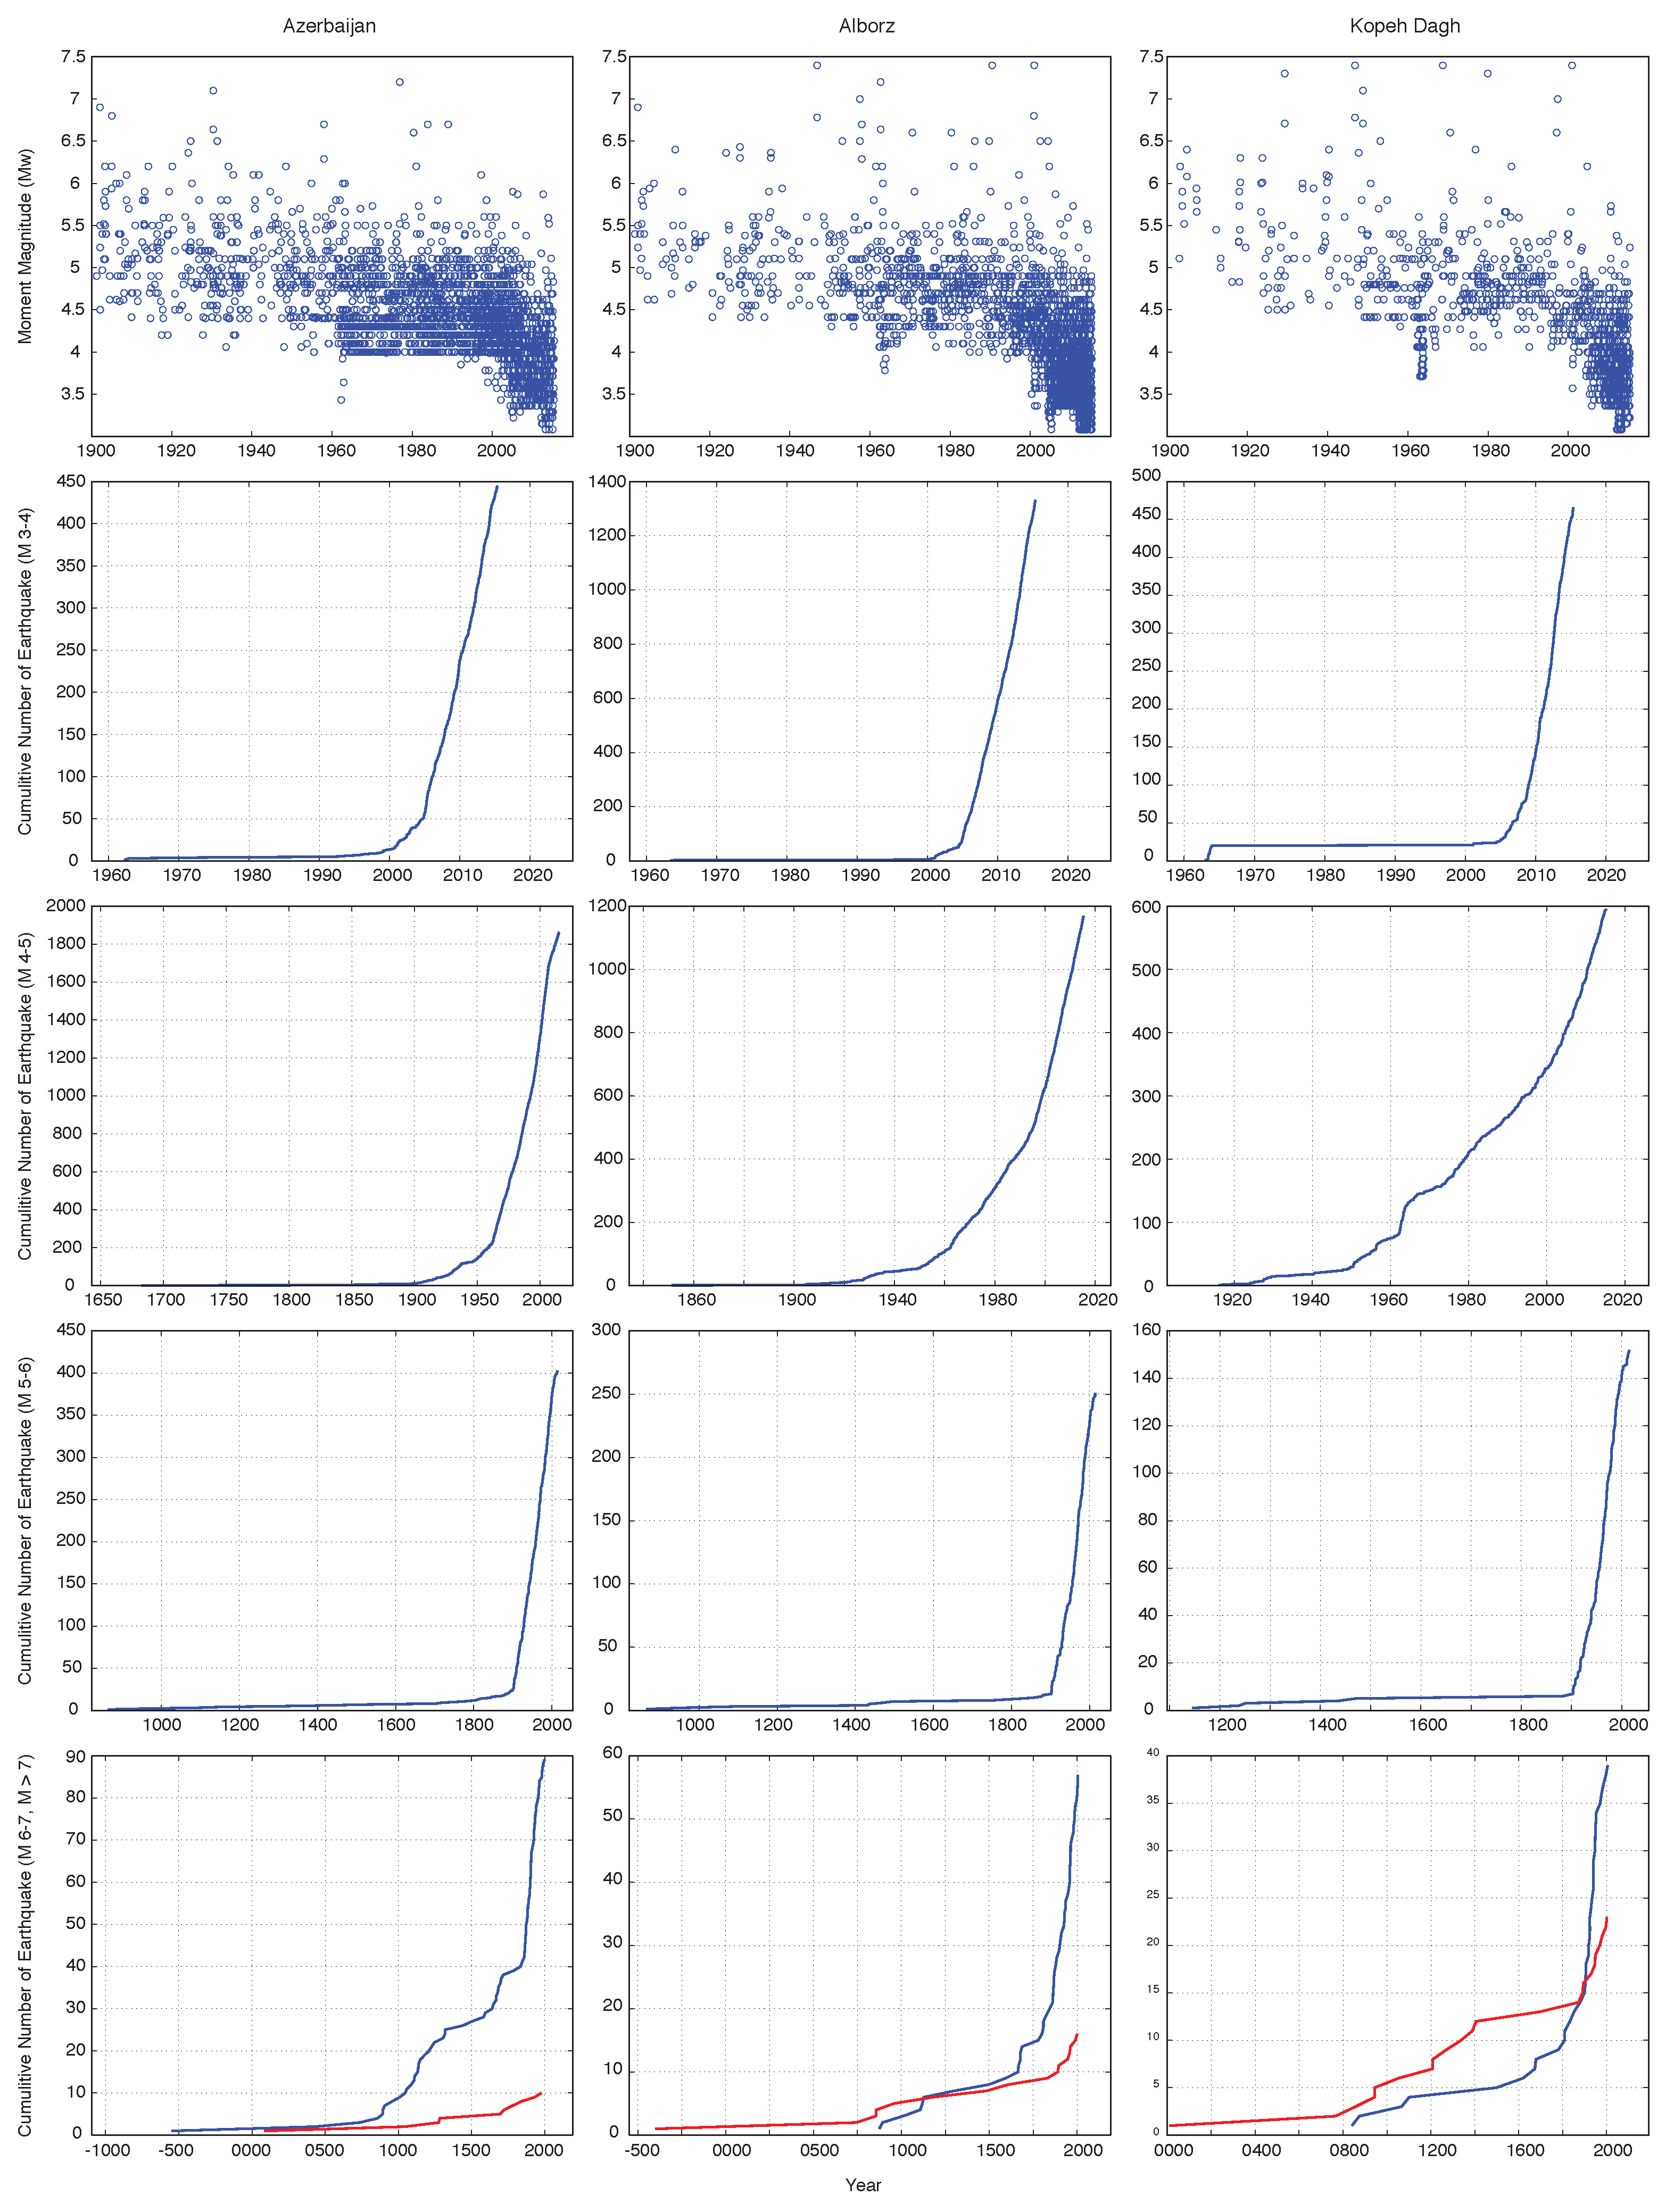
\includegraphics[scale=0.3]{figures/pdf/Figure4.pdf} 
\caption{Completeness test for earthquakes occurred in the three study regions. Red lines represent $M_w > 7$ }
\label{fig:comptest}
\end{figure*}



\begin{table}[h]
\centering
\caption{Completeness threshold of three tectonic seismic regions.}
\begin{tabular}{cccc}
 ~           & Azerbaijan & Alborz & Kopeh Dagh \\ \hline
3-4         & 2004       & 2004   & 2005       \\ \hline
4-5         & 1960       & 1960   & 1960       \\ \hline
5-6         & 1900       & 1900   & 1900       \\ \hline
6-7         & 1844       & 1809   & 1810         \\ \hline
7 $< $    &  85          & -400    & 10         \\ \hline
\end{tabular}
\end{table}
